% vim: ts=2:sw=2:tw=80:et
\thispagestyle{fancy}
\pagestyle{fancy}

\begin{figure}[htb!]
  \centerline{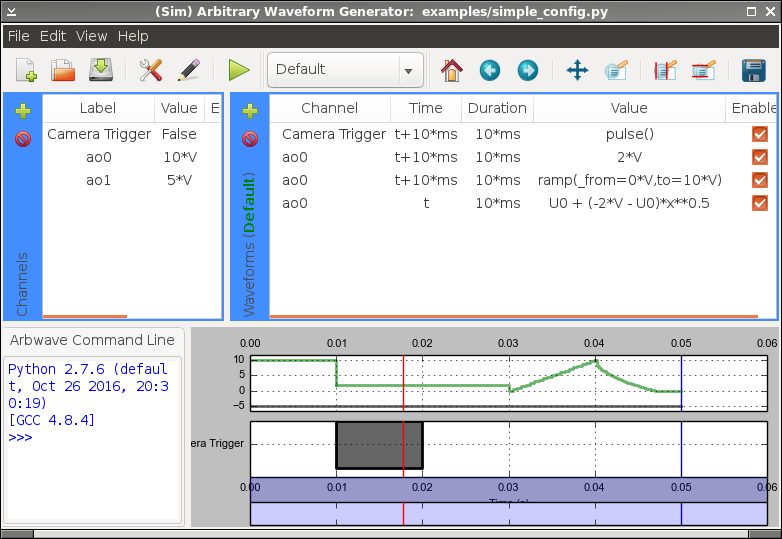
\includegraphics[width=.8\textwidth]{figures/main-simple-config}}
  \caption{Main window when initially loading ``simple-config.py'' in simulated
  mode.}
  \label{fig:quick:main-simple-config}
\end{figure}


In order to get at least a quick feel of what Arbwave is like, it can be very
helpful to run in Simulated Mode with one of the packaged examples.

To do this, use the \verb|--simulated| command line.  There are two ways for you
to load up one of the examples.
\begin{enumerate}
  \item Add the filename of one of the examples on the command line, such as:\\
    \begin{verbatim}
    run.py --simulated examples/simple_config.py
    \end{verbatim}
    or perhaps:
    \begin{verbatim}
    run.py --simulated examples/simple_ni_only_config.py
    \end{verbatim}
  \item Start Arbave up in simulated mode with \verb|run.py --simulated| and
  then use the Open menu option.  Browse to \verb|examples/| and select one of
  the included examples.
\end{enumerate}
%
After loading the \verb|simple_config.py| example, you should see the main
window as shown in Fig.~\ref{fig:quick:main-simple-config}.  The simulated
waveforms can be modified to explore Arbwave capabilities.
